\documentclass[12pt]{article}
\usepackage{amsfonts, epsfig}
\usepackage[authoryear]{natbib}
\usepackage{graphicx}
\usepackage{fancyhdr}
\pagestyle{fancy}
\lfoot{\texttt{comsm0021.github.io}}
\lhead{Neural Information Processing - 8\_forward\_models - Conor}
\rhead{\thepage}
\cfoot{}
\begin{document}

\section*{A forward model for the perception of movement}

In neuroscience, and in control theory, a \textsl{forward model} is an
internal model responsible for what performing calculations analagous
to the dead reckoning discussed in the context of Kalman filters.

A well-known discussion of forward models in given in
\cite{WolpertEtAl1995}. In this paper they give some, albeit quite
circumstantial, evidence that the brain has a forward model for
movement. In their experiment subjects are sat in the dark with one
hand on a manipulandum, that is, a device you push around with one
hand which can record your hand, restrict it to specific paths and
excert a force against or with the movement of your hand. A
manipulandum is shown in Fig.~\ref{fig_manipulandum}.

In this experiment the manipulandum is restricted to horizonal
motion. At the start of each trial the location of the subjects hand
is illuminated and it is assumed that at that time the subject knows
exactly where their hand is. The subject is then asked to move their
hand; there may be a force assisting or resisting this movement, in
any case at the end a restiance force is used to force the subject to
stop moving there hand at a point uniformly chosen between zero and 30
cm.  The subject is then asked to use their other hand to indicate,
using a mouse which moves a marker along the horizonal track, where
they believe where their hand is. It turns our people consistiently
over-estimate how far their hand has travelled.\footnote{This raises a
  plethora of questions; like if they then get visual feedback does
  the estimate improve? Is the overestimate the result of not
  modelling the braking force? This isn't dealt with in the paper and
  may work against its conclusions!}  In fact this overestimate has a
distinctive timecourse shown in Fig.~\ref{fig_overestimate}: the
overestimate increases rapidly for movements that take a second or
less and then descreases slowly for longer movements.


\begin{figure}{htb}
\begin{center}
  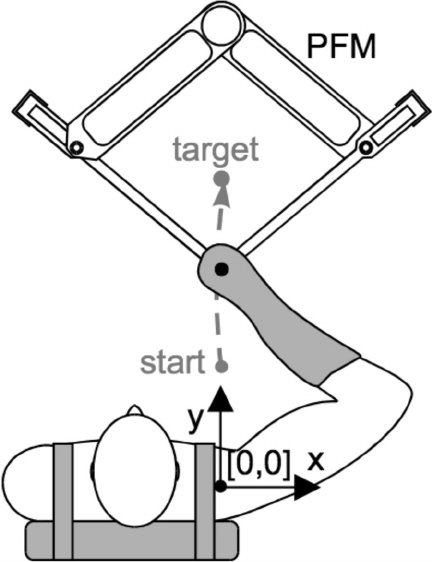
\includegraphics[width=6cm]{manipulandum.jpg}
\end{center}
\caption{A manipulandum allows hand movements to be recorded and to be
  manipulated by applying a force. [Image from \cite{MistryEt2013},
    the start and target labels don't apply to the experiment being
    discussed here].\label{fig_manipulandum}}
\end{figure}


\begin{figure}{htb}
\begin{center}
  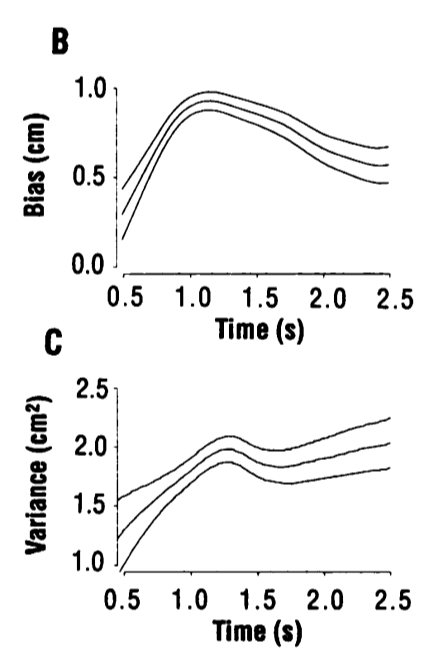
\includegraphics[width=5cm]{fig_overestimate.png}
\end{center}
\caption{The bias in estimates of hand position; \textbf{B} shows the
  mean bias and \textbf{C} the mean variance. The middle line shows
  the mean and the two outer lines are standard errors indicating the
  variability of the measurement. The participants never stop moving
  their hands in less than 0.5 seconds so the graphs start there;
  after 2.5 second the bias stops changing; 1 second corresponds to
  0.9 cm and 2.5 seconds to 2 cm. [Image from
    \cite{WolpertEtAl1995}].\label{fig_manipulandum}}
\end{figure}

It is proposed in \cite{WolpertEtAl1995} that this is evidence for a
forward model. In there description the sense of hand position in the
absence of visual feedback has two components, a dead reckoning
component supplied by the forward model and a proprioceptive component
coming from mechano-receptors and joint receptors in the arm
itself. The dead reckoning model is similar to what we saw before for
the Kalman filter:
\begin{equation}
\mathbf{x}_d=F\textbf{x}+U(t)\textbf{c}+\textbf{W}
\end{equation}
where, as before 
\begin{equation}
F=\left(\begin{array}{cc}1&t\\0&1\end{array}\right)
\end{equation}
but here there is in addition a control vector corresponding to the
force the subject applies to the manipulandum. 
\begin{equation}
\textbf{c}=\left(\begin{array}{c} 0\\1/m\end{array}\right)
\end{equation}
and $U(t)$ is the work done on the manipulandum, so $U(t)=\int_0^t
u(t)dt$ where $u(t)$ is the force on the manipulandum, both from the
subject and, possibiliy, from the added force applied to the
manipulandum during the experiment. Finally $\textbf{W}$ is the
noise. Basically, the difference from what we saw before is the extra
control term modelling the accelleration of the manipulandum. In this
picture this force is something the brain knows about, they are the
motor commands whose effect is begin modelled. In any case, the
details here are not important, the main thing is that in this model
the brain models the consequence of the motor commands and produces a
prediction based on dead reckoning of where the hand is. One detail is
important, the covariance of $\mathbf{W}$ grows with time, if $W$ is
the covariance matrix then $W=wt$ for some $w$.

Overall the model has a prediction from the forward model and sensory
information from proprioception; these are combined to give a new
estimate of the position $\mathbf{x}_n$
\begin{equation}
\mathbf{x}_n=\textbf{x}_d+K(\textbf{x}_s-\textbf{x}_d)
\end{equation}
where $\mathbf{x}_s$ is the sensory estimate of the position and $K$
is the Kalman gain.\footnote{All this is described in position space,
  as if in the brain the sensory information is converted into
  position information; a more likely picture is that the forward
  model outputs a sensory prediction. However, this doesn't change the
  picture being presented here.}

In this picture of motor control the movement of the hand is under
continouous feedback control; as the hand is moving the forward model
is predicting where the hand will soon be so the motor areas can issue
instructions for what the muscles must do next to move from that point
to the one beyond. This continuous feedback is a more adaptible and
robust model of motor control than one involving a backward model; in
a backward model the desired final location of the hand is the input
and the output is the required motor commands. 




\bibliographystyle{apa} \bibliography{../../source/bibliography}{}



\end{document}

